\section{Background}
\label{sec:Background}

\subsection{Introduction}

High Performance Computing (HPC) initiatives over the past decade have 
fostered the development of extremely successful scalable analysis tools ---
such as ParaView, VisIt, and Ensight --- that make it possible to visualize 
and explore very large datasets.  This success provides a foundation for 
the analysis we will do at Exascale, but the core disruptions caused by
the push to Exasacle --- disrutptions that will be experienced by the entire
software stack, as well as the science codes --- will force us to fundamentally
change how we do \vda in the years ahead.

Current visualization and data analysis is largely done as an off-line
post-processing step, in which interactive visualization tools read in data
saved to disk, and an analyst sitting at a desk interacts with that data in
real time.  This method uses the disk as a communication mechanism between
the science code and the \vda application, so the code and interactive
analysis are functionally decoupled.  There are some efforts aimed at
changing this workflow, but it remains the standard way that people
interact with their data.

At extreme scale, current workflows will be completely broken due to 
the mismatch
between the rate at which we can create large data, and the rate at
which that data can be moved to persistent storage.  In fact, this
data movement will be so costly in terms of energy that it will be
cost prohibitive to move results from memory to persistent storage.
Because of this, extreme scale computing will have integrated \vda as a
method of determining what data are of interest and therefore worth
committing to persistent storage.

This data can be visualized interactively, analyzed,
sent to a data-centric computation, or written to persistent
storage.  Depending upon the needs of the end-user analysis, one or
more of these data collaboration steps may be requested.  The design
of the computation system --- from compute architecture through system
software and persistent storage model --- will be determined by the
needs of the analysis being performed at the end of the compute
cycle.  This sytem level co-design must take into account the
constraints of the compute resources (power, time, and cost), as
well as the requirements of the science and exploration to be done
at the conclusion of the scientific simulation.

\subsection{Current Post-Processing Pipelines}

The current prevalent practice of computational-based scientific analysis
is a progression of relatively independent steps.  First is a problem
setup, which involves setting up initial and boundary conditions,
determining materials and their properties, and creating a mesh or
establishing a meshing proceedure.  Based on this problem setup, a
simulation is next run.  During the progression of the simulation, results
files are periodically recorded to disk storage.  This results data are
typically the geometry of physical entities being simulated (often but not
always a mesh of finite elements) with field values of physical properties
given for the topological units of the geometry.  Because of limitations
with disk storage bandwidth and capacity, results data seldom capture all
computed interations but rather capture data at some periodicity specified
by the analyst.  At some time later, a \vda job reads this data back from
disk and presents an interactive analysis session with a user.

This ``off-line'' post-processing \vda offers many advantages that make it
the easiest way to perform visualization.  First, because the simulation
and visualization are run in completely different jobs and nominally at
different times, the \vda requires no additional resource overhead on the
simulation (other than the requisite storage of results to disk).  Second,
it makes the interface between simulation and visualization simple.  The
visualization needs only to understand the format used when the simulation
writes the data to disk.  Third, it makes scheduling and performing the
visualization, particularly when done by a human, much easier.  The
visualization job can be scheduled completely independently of the
simulation and at a time most convenient to the user.  Fourth, the results
data are placed in persistent storage, so any analysis not performed
immediately can be done at a later time if they are later deemed necessary.
Thus, when it is feasible, off-line post-processing is a convienient and
effective mechanism for \vda.

\subsection{Extreme-scale Analysis: New Challenges}
\label{sec:NewChallenges}

\fix{Ken wants to revisit this.}


\begin{figure}
\begin{center}
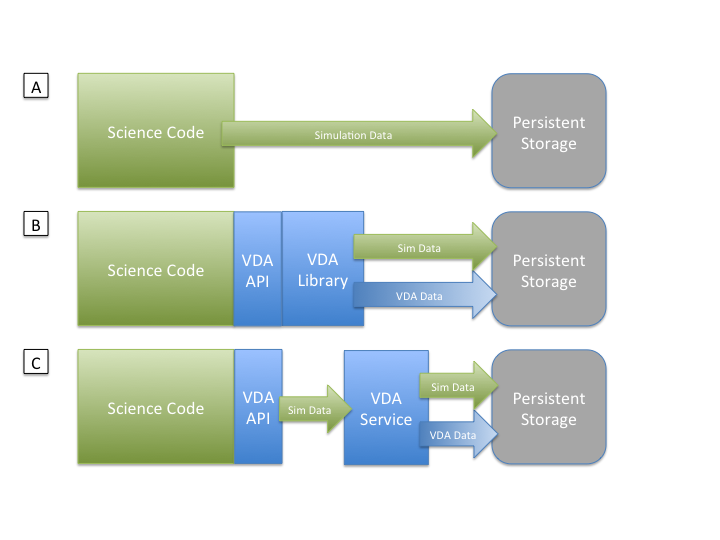
\includegraphics[width=6in]{figures/three-data-flows}
\end{center}
\caption{ A simplified pipeline diagram showing the flow of information from simulation to persistent storage in one example of a modeling and simulation workflow (we note that writing to persistent storage is not the only end state of analysis, as is explained WHERE).  Most data analysis today occurs as a \emph{post-processing} step, as in pipeline \textbf{A}.  However, as we move to extreme scale science, we must adopt workflows that integrate \vda more closely, either as in pipeline \textbf{B}, as a library compiled into the simulation code, or as in pipeline \textbf{C}, as a loosely coupled service.  In either case, we expect a standard \vda API to be used by the science code, so that \vda code can be executed efficiently according to the hardware and execution policy available.
\label{simplepipeline}}
\end{figure}

Why is science at Extreme Scale so different from current practice?  Can't we
continue using the successfully deployed applications for this new scale, if, like science codes, we adapt to the challenges of the new architectures?

The answer is, simply, no.  A major challenge moving from current architectures to extreme architectures and extreme scales are twofold.  First, the rate of 
computation far outstrips the rate of I/O for a large system.  Second, it is
prohibitively expensive in terms of power to move large datasets from memory,
across networks, to disks.  These two considerations, spelled out in detail in
HERE HERE and HERE, require us to alter our current analysis pipeline.

More importantly, there are system wide implications resulting from the solution
to this problem, which include domain and technique specifc analysis techniques,
in-situ framework development, and complexity impacts in post-processing.

Figure~\ref{simplepipeline} shows simplified diagrams showing the flow of information from simulation to persistent storage in a typical modeling and simulation workflow.  Typical \vda occurs as a 'post processing' step, after the simulation has written results directly to persistent storage.  Typically, these results are in a code-specific format, and are formatted as 'restart' files - optimized for reading back into an instance of the science code, and not optimized for post processing analysis by \vda tools.  Extreme computation size and extreme architectures force data flows like (b) and (c), in which \vda is performed on the simulation results before they are written to persistent storage.  In (b), data is handed directly to a \vda library coupled with the running code.  In (c), data are 'sent' to \vda process separate from the running code, enabling analysis, visualization and data reduction under the control of the science code - at the cost of sharing runtime resources with the \vda execution.  This decouples the data computation and \vda processes, which affords many advantages, at the cost of system complexity.  Both approaches must be provided for extreme scale analysis, so that the codes, system designers, and science customers can design a computation and analysis workflow suited to the specific needs of the science, analysis and decision support being supported.


\subsection{Motivation}

\fix{``Motivation'' is probably already covered in
  Section~\ref{sec:NewChallenges} that Dave just added.  Perhaps rather
  than Motivation this should be a brief summary of our approach to the
  solution, to be expanded on in Sections \ref{sec:Catalyst},
  \ref{sec:Nessie}, and \ref{sec:UseCase}.}

\fix{Some motivating discussion can be found in this workshop
  report:~\cite{ScientificDiscoveryExascale2011}.}

\subsubsection{Catalyst}

\subsubsection{Nessie}
